\documentclass[a4paper,10pt]{article}
\usepackage[T1]{fontenc}
\usepackage[utf8]{inputenc}
\usepackage[english]{babel}
\usepackage{lmodern}
\usepackage[top=1.6cm,bottom=1.8cm,left=1.9cm,right=1.9cm]{geometry}
\usepackage{titlesec,enumitem,xcolor,graphicx,lastpage,fancyhdr}
\usepackage{fontawesome5}
\usepackage[hidelinks]{hyperref}

\hypersetup{colorlinks=true,urlcolor=blue!70!black,linkcolor=blue!70!black}
\pagestyle{fancy}\fancyhf{}\renewcommand{\headrulewidth}{0pt}
\fancyfoot[C]{\small\color{gray}Page \thepage\ of \pageref{LastPage}}
\setlength{\parindent}{0pt}

\titleformat{\section}{\large\bfseries\color{blue!70!black}}{}{0em}{}[\vspace{-0.7em}\rule{\textwidth}{0.5pt}]
\titlespacing{\section}{0pt}{9pt}{5pt}
\setlist[itemize]{leftmargin=1.1em,itemsep=2pt,topsep=2pt,parsep=0pt}
\newcommand{\role}[4]{\vspace{3pt}\noindent\hspace{0.6em}\parbox[t]{0.38\textwidth}{\raggedright\textbf{#1}}\hfill\parbox[t]{0.58\textwidth}{\raggedleft\textit{#2}}\\{\textit{#3}\hfill\textit{#4}}\vspace{1pt}}

\begin{document}
\noindent
\begin{minipage}[t]{0.78\textwidth}
\vspace{0pt}
{\huge\bfseries Prabhavit Gupta}\\[8pt]
{\small \faPhone\ +39-351-610-7807 \quad \faEnvelope\ \href{mailto:prabhavitg@gmail.com}{prabhavitg@gmail.com} \quad \faLinkedin\ \href{https://www.linkedin.com/in/prabhavit/}{Linkedin} \quad \faMapMarker*\ Venice, Italy}
\end{minipage}\hfill
\begin{minipage}[t]{0.18\textwidth}
\vspace{0pt}\raggedleft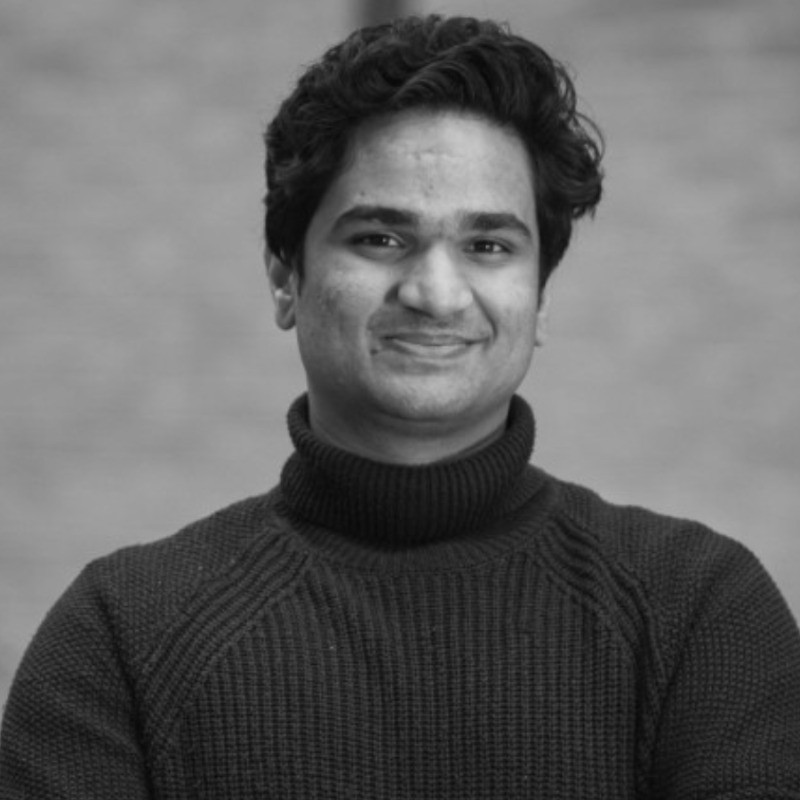
\includegraphics[width=2.3cm,height=2.3cm,keepaspectratio]{photo.jpg}
\end{minipage}

\section{Career Summary}
\begin{itemize}
\item IoT Platform \& Systems Integration Engineer with dual degrees in Mechanical Engineering and Management Engineering (Politecnico di Milano).
\item Solid foundation in architecting and operating industrial IoT platforms, bridging manufacturing shop-floor assets (OT) with enterprise cloud applications (IT).
\item Extensive hands-on experience implementing MQTT message brokers, OPC UA servers/clients, Modbus protocols, and real-time streaming pipelines.
\item Proficient in dashboard engineering and metrics visualization using Grafana, Prometheus, and Elasticsearch, paired with automated Python edge services.
\end{itemize}

\section{Technical Skills}
\begin{itemize}
\item \textbf{IoT Protocols \& Connectivity} -- MQTT (EMQX, Mosquitto), OPC UA, Modbus TCP/RTU, WebSockets, REST APIs, Webhooks, HTTP/2
\item \textbf{IT/OT Convergence \& Architecture} -- Edge Gateways, Fieldbus Integration, Industrial Ethernet, Network Segregation, Microservices
\item \textbf{Observability \& Visualization} -- Grafana, InfluxDB, Prometheus, Elasticsearch, Logstash, Kibana (ELK), Time-Series Data Modeling
\item \textbf{Software \& Scripting} -- Python, TypeScript, Bash, SQL, NoSQL (MongoDB, Redis), Docker, Linux, Git, CI/CD
\item \textbf{Methodology \& Tools} -- Agile/Scrum, Atlassian Suite (Jira, Confluence), Technical Runbooks, Incident Troubleshooting
\end{itemize}

\section{Visa \& Language}
\begin{itemize}
\item \textbf{Language} -- English (Fluent / Professional), Italian (Conversational / Intermediate), Hindi (Native)
\item \textbf{Work Authorization} -- European Long Term Residence Permit (No Visa Sponsorship required). Driving License (Patente B). Available for Bologna hybrid schedule.
\end{itemize}

\section{Professional Experience}
\role{\href{https://flowspace.co}{FlowSpace.co}}{IoT Platform \& Integration Lead}{London, UK / Remote}{Mar 2024 -- Ongoing}
\begin{itemize}
\item \textbf{IoT Platform Architecture \& Data Pipelines:}
\begin{itemize}[label=--]
\item Architected high-throughput telemetry ingestion services utilizing MQTT and WebSockets, routing streaming machine metrics to backend data stores.
\item Built real-time monitoring dashboards in Grafana tracking connected device status, signal latencies, and payload throughput across distributed deployments.
\item Integrated edge hardware with central cloud microservices via secure REST endpoints and containerized gateway proxies.
\end{itemize}
\item \textbf{System Reliability \& Agile Collaboration:}
\begin{itemize}[label=--]
\item Coordinated cross-functional sprint deliveries following Agile workflows across Jira and Confluence, accelerating release cadence.
\item Maintained 99.9\% uptime across telemetry collectors through automated alerting, failover routines, and continuous health probes.
\end{itemize}
\item \textit{Tools: MQTT, OPC UA, Grafana, Python, Docker, Linux, NoSQL, Git, Jira}
\end{itemize}

\role{Urlink}{Systems Automation Engineer}{Milan, Italy}{Jul 2023 -- Feb 2024}
\begin{itemize}
\item Configured industrial IoT edge gateways to extract machine state parameters from PLCs over Modbus and OPC UA.
\item Integrated field sensors into centralized operational databases, validating data integrity during client plant commissioning.
\item Drafted protocol configuration documentation, interface mapping tables, and network troubleshooting checklists.
\end{itemize}

\role{UltraStrategy}{Automation Developer}{Remote, Germany}{Sep 2022 -- Jun 2023}
\begin{itemize}
\item Developed Python automation scripts extracting operational time-series data from connected sensors and machinery.
\item Designed automated reporting pipelines summarizing daily production throughput and sensor deviation alerts.
\end{itemize}

\section{Education}
\role{Politecnico di Milano}{M.Sc. in Management Engineering (Digital Business \& ICT)}{Milan, Italy}{2020 -- 2023}
\role{Thapar Institute of Engineering and Technology}{B.E. in Mechanical Engineering}{Punjab, India}{2014 -- 2018}

\end{document}
